\documentclass[10pt]{article}

\usepackage[margin=1in]{geometry}
\usepackage{amsmath}
\usepackage{booktabs}
\usepackage{graphicx}
\usepackage{microtype}
\usepackage{placeins}
\usepackage[hidelinks]{hyperref}
\usepackage{xcolor}

\newcommand{\pisti}{Pişti}
\newcommand{\code}[1]{\texttt{#1}}
\newcommand{\DirectMean}{2.66}
\newcommand{\DirectMedian}{2.76}
\newcommand{\DirectCILow}{2.41}
\newcommand{\DirectCIHigh}{2.90}
\newcommand{\DirectBootLow}{2.16}
\newcommand{\DirectBootHigh}{3.15}
\newcommand{\DirectP}{0.0020}
\newcommand{\DirectPositive}{10}
\newcommand{\DirectWinRate}{0.564}
\newcommand{\DirectPistiDiff}{0.180}
\newcommand{\DirectCapturedDiff}{3.35}
\newcommand{\AcuteMean}{2.63}
\newcommand{\AcuteCILow}{2.29}
\newcommand{\AcuteCIHigh}{2.98}
\newcommand{\AcuteP}{0.0020}
\newcommand{\AcutePositive}{10}
\newcommand{\AdaptMean}{-0.02}
\newcommand{\AdaptP}{0.8828}
\newcommand{\StochasticMean}{2.38}
\newcommand{\StochasticCILow}{2.19}
\newcommand{\StochasticCIHigh}{2.57}
\newcommand{\StochasticP}{0.0020}
\newcommand{\AnchorMean}{2.41}
\newcommand{\AnchorP}{0.0020}
\newcommand{\RatingDiff}{42.6}
\newcommand{\RobustnessMean}{-0.19}
\newcommand{\RobustnessCILow}{-0.97}
\newcommand{\RobustnessCIHigh}{0.60}
\newcommand{\RobustnessP}{0.6250}
\newcommand{\RobustnessPositive}{2}
\newcommand{\PrincipalMax}{0.98}


\title{What Is Played-Card Memory Worth?\\
A Seed-Replicated Self-Play Study in \pisti}
\author{Anonymous Author(s)}
\date{}

\begin{document}
\maketitle

\begin{abstract}
Card counting is considered central to skilled play in many imperfect-information card games, yet learned policies are often given a complete action history without measuring its value. We study this question in \pisti, a Turkish capture game with a small action space, hidden hands and stock, and strategically important played-card identities. We implement and test a two-player environment, then train Maskable PPO policies for six million environment steps under a curriculum and snapshot league. The confirmatory experiment uses ten paired training seeds that differ only in whether a 52-dimensional vector of observed cards is available. Every comparison replays 500 independently generated deals with both seat assignments. We additionally remove memory from trained policies at inference, evaluate stochastic policies and common anchors, and train fixed-budget approximate best responses against league and fixed-opponent controls. Explicit memory changed direct head-to-head score by \DirectMean{} points per game (95\% seed-level interval \DirectCILow{} to \DirectCIHigh{}; exact sign-flip $p=\DirectP$). Acute removal changed score by \AcuteMean{} points per game, separating reliance on the feature from adaptation during training. The agreement between retrained and acute interventions shows a large, seed-consistent benefit from exact played-card identity history under this policy class and protocol. The contribution is empirical and domain-specific: it quantifies a representation choice and provides a reproducible \pisti{} benchmark, but does not claim algorithmic novelty or equilibrium convergence.
\end{abstract}

\section{Introduction}

Imperfect-information games are useful laboratories for sequential decision making because a policy must act on an information set rather than a fully observed state. Modern methods can learn strong play from self-play, but their performance depends on what the observation makes easy to remember. In card games, a vector of previously observed cards is a common engineering choice. It is also a substantive assumption: it grants exact recall while avoiding the burden of learning memory in a recurrent network.

We ask a narrow causal question: how much does this explicit played-card memory improve learned play in \pisti? \pisti{} is well suited to the question. Captures depend only on the current top card, while the value of discards and the likelihood that ranks remain in hidden locations depend on play history. A feed-forward policy can act legally from its hand and the table top without history, but it cannot explicitly count which cards have disappeared. The game therefore separates immediate tactical information from historical information without a large or variable action language.

The repository originally contained a broad exploratory study with PPO, DQN, neural fictitious self-play, search baselines, mirrored tournaments, and approximate exploitability. That evidence was useful for hypothesis generation but insufficient for a paper-level memory claim: the full-memory and no-memory agents were not paired by seed, training uncertainty was underrepresented, and historical results were produced under a slightly different rule implementation. We therefore used a structured literature review and an evidence audit to select the experiment before examining new outcomes. The review found established work on self-play, equilibrium learning, card-game toolkits, and information-set search, but no directly relevant \pisti{} AI paper under the documented search protocol. It did not support an algorithmic-novelty claim. It did support a focused representation study and a tested benchmark.

This work makes three contributions:
\begin{enumerate}
    \item a ten-seed paired estimate of the value of explicit played-card memory, with inference over training seeds rather than treating games as independent runs;
    \item a distinction between retraining without memory and acutely removing memory from an already trained policy, plus deterministic, stochastic, anchor, and cross-play sensitivity analyses; and
    \item an open, rule-tested \pisti{} environment with duplicate-deal evaluation and replicated fixed-budget attacks that are reported as lower bounds on exploitability.
\end{enumerate}

\section{Background and Related Work}

We conducted a structured scoping review on 8 August 2026 using English and Turkish search families for \pisti, related fishing games, imperfect-information self-play, information-set search, exploitability, and empirical RL design. We screened scholarly pages and primary records from arXiv, ACM, IEEE, Springer, IJCAI, PMLR, JMLR, OpenReview, and citation metadata, then used backward and forward snowballing until two rounds added no new contribution category. Twenty-six works were retained in the evidence matrix. No directly relevant \pisti{} AI study was found under this protocol; this is a search result, not a universal absence claim.

\subsection{The game}

\pisti{} is played with a standard 52-card deck. Four cards initialize the center, one face up and three face down, and each player receives four cards. Players alternately add one card to the face-up pile. A card captures the pile when its rank matches the previous top card; a Jack captures any nonempty pile. A rank match against a one-card pile scores a ten-point pişti bonus, while Jack on Jack scores twenty in the implemented variant. The first capture also collects the initially hidden center cards, which are privately inspectable by that capturer. After both hands empty, packets of four are dealt until all cards are played. Remaining table cards go to the last capturer. Aces and Jacks score one point each, the two of Clubs scores two, the ten of Diamonds scores three, and a strict majority of captured cards scores three. The first capture and final play cannot score pişti \cite{pagatpisti}.

The game is finite, two-player, zero-sum in score differential, and imperfect-information. At a decision, a player knows its hand, all face-up play, public capture counts and bonuses, and any center cards it personally collected. It does not know the opponent's hand, the stock order, or center cards collected by the opponent. Our opening procedure swaps an opening Jack with a non-Jack among the four center cards; an all-Jack center triggers a redeal. This explicit implementation choice avoids an initial Jack and is held constant across all conditions.

\subsection{Learning and search in imperfect-information games}

Counterfactual regret minimization provides convergence guarantees in finite extensive-form games when regrets can be traversed or approximated \cite{zinkevich2007cfr}; Deep CFR replaces tabular regrets with function approximation \cite{brown2019deepcfr}. Neural fictitious self-play combines an approximate best response with a learned average policy \cite{heinrich2016nfsp}. Population-based response-oracle methods formalize strategy populations and meta-games \cite{lanctot2017psro}, while ReBeL integrates belief-state learning and search with guarantees in two-player zero-sum games under its assumptions \cite{brown2020rebel}. These approaches establish an important boundary for our claims: ordinary PPO self-play can produce a useful policy, but its returns do not demonstrate convergence to a Nash equilibrium.

OpenSpiel and RLCard have made standardized game environments, baselines, and evaluation practices central to card-game research \cite{lanctot2019openspiel,zha2020rlcard}. In the closest game-family study we found, Di Palma and Lanzi compared rules, MCTS, and information-set MCTS in Scopone and showed why fair information-set search must be separated from access to hidden state \cite{dipalma2018scopone}. Information-set MCTS more generally addresses pathologies of independent determinizations \cite{cowling2012ismcts}. Our search anchor samples legal determinizations and is useful as a common opponent, but is not presented as a new or theoretically sound equilibrium solver.

\subsection{Empirical design}

Deep RL is sensitive to seeds, implementations, and reporting choices \cite{henderson2018matters}. Deal-level confidence intervals quantify evaluation noise for a fixed trained policy; they do not quantify the training procedure's variation. Recommendations for few-run RL experiments therefore emphasize independent training runs, uncertainty intervals, and transparent aggregation \cite{agarwal2021precipice,patterson2024empirical}. We use ten paired training seeds and make the seed, not an individual game, the independent unit for the primary claim.

Random deals create a second source of variation. Duplicate tournaments replay the same random deal with assignments swapped, allowing deal luck to be canceled in a paired comparison \cite{yu1995duplicate}. All main matches here use this design. Finally, learned best responses can reveal failures that average opponents miss, but in large games they estimate only a lower bound on exploitability \cite{timbers2022exploitability}. We consequently use the term \emph{discovered attack edge}, never exact exploitability.

\section{Methods}

\subsection{Environment and observations}

Cards are represented as integers from 0 to 51. The engine exposes legal actions, cloning, and information-set determinization. Tests cover golden rule cases, card conservation, scoring conservation, reward telescoping, mirrored seating, private center-card knowledge, determinization, and observation-space validity. The policy receives a dictionary observation containing: (i) a 52-dimensional multi-hot hand; (ii) a 52-dimensional one-hot table top; (iii) a 52-dimensional \code{seen} vector; (iv) 12 normalized public or privately known scalar statistics; and (v) a legal-action mask. Scalar point features exclude the value of center cards privately held by the opponent. Statistics are clipped to the declared range.

The memory treatment changes only \code{seen}. In the memory condition it contains the initial upcard, every face-up played card, the current hand, and the three initial center cards after the observing player captures them. In the no-memory condition it is identically zero. Hand, current table top, capture counts, known point totals, pişti counts, and last-capturer indicators remain available. Thus ``no memory'' means no explicit card-identity history, not a stateless or fully amnesic player. Both the learner and frozen self-play opponents receive the condition-appropriate observer.

The environment's dense reward is the change in the learning player's score differential between consecutive decisions, scaled by 0.1. Its undiscounted episode sum telescopes exactly to 0.1 times terminal score differential. PPO uses $\gamma=0.999$, so training introduces a small temporal weighting of those increments; this choice is held fixed across conditions.

\subsection{Training}

All primary policies use PPO \cite{schulman2017ppo} with invalid actions masked \cite{huang2020masking} and a two-layer multilayer perceptron of 256 units per layer. Each run uses eight synchronous environments, learning rate $3\times10^{-4}$, rollout length 256 per environment, batch size 512, four epochs, $\gamma=0.999$, GAE parameter 0.95, clipping 0.2, entropy coefficient 0.01, and six million environment steps.

The opponent curriculum begins with equal random and greedy play. At 300k steps it switches to 0.6 greedy and 0.4 pişti-hunter. At one million steps it uses 0.2 greedy, 0.2 hunter, 0.4 historical snapshot, and 0.2 current policy. At 2.5 million it uses 0.1 each greedy, hunter, and light determinization search, 0.45 snapshots, and 0.25 current policy. Snapshots are taken every 250k steps and a random-replacement pool retains at most 12. Memory-on and memory-off policies are trained from scratch for seeds 0--9 with otherwise identical configurations.

For the secondary league comparison, five additional full-memory policies use the same first two phases and total step budget. At later phases, self-play components are removed and the remaining scripted weights are renormalized: equal greedy/hunter weights at one million steps and equal greedy/hunter/search weights at 2.5 million.

\subsection{Evaluation}

Every main matchup uses 500 decks drawn from a fixed evaluation seed. Each deck is played twice, swapping which policy receives the leading seat and corresponding card packets, for 1,000 games per matchup. Policies act deterministically unless a sensitivity analysis is explicitly labeled stochastic.

The primary comparison matches memory-on seed $s$ directly against memory-off seed $s$ for all ten seeds. The acute ablation matches two copies of each memory-trained model, giving one its ordinary observer and zeroing \code{seen} for the other. This estimates reliance by a policy that did not adapt to feature removal. We also repeat direct matches with stochastic action sampling, evaluate every policy against greedy, hunter, and 16-sample determinization-search anchors, and run a 20-policy cross-play tournament. The stochastic sampling seed is fixed as the evaluation seed plus the training seed.

\subsection{Statistical analysis}

For a policy pair and deal $d$, let $y_{d,1}$ and $y_{d,2}$ denote score differentials from the two seat assignments. The duplicate-deal effect is $z_d=(y_{d,1}+y_{d,2})/2$. For each training seed we average its 500 $z_d$ values. H1's effect is the mean of the ten seed effects. We report every seed effect, the mean and median, a Student-$t$ interval over seeds, and an exact two-sided sign-flip permutation test over the $2^{10}$ possible signs. Because all policies reuse the same decks, training seed and evaluation deal are crossed factors; a two-way bootstrap resamples seed indices and shared deal indices. The preregistered descriptive labels are small below 0.5 points per game, moderate from 0.5 to 1.5, and large above 1.5; these are conventions, not human-calibrated thresholds.

The same seed-level procedure is applied to acute removal and stochastic sensitivity. H3 uses the within-seed acute effect minus the retrained direct effect. Anchor results first average score differentials across the three anchors within each seed and condition. Cross-play Bradley--Terry ratings \cite{bradley1952rank} are descriptive because pairwise match records reuse policies and deals.

H1 is the sole primary test. P-values for H2--H4 and sensitivity analyses are reported as unadjusted secondary evidence and interpreted together with effect sizes and intervals, not as a family of independent confirmatory discoveries.

\subsection{Fixed-budget attacks}

For target seeds 0--4, we train a Maskable PPO attacker for one million steps against the stochastic frozen league policy and its seed-matched fixed-opponent control. Both attackers start from the same historical PPO checkpoint, use attacker seed $100+s$, and are evaluated with 500 mirrored deals. Two additional attackers with seeds 201 and 202 target league seed 0. We report each edge, the maximum discovered edge for the replicated target, and the paired fixed-minus-league difference over five target seeds. These are budget- and attacker-dependent lower bounds, not exact best responses.

\subsection{Protocol integrity and reproducibility}

The hypotheses and analysis were frozen after a timing pilot and before completed confirmatory outcomes. The earlier exploratory report motivated the questions, so this is a confirmatory replication and extension rather than pristine preregistration. A pre-outcome rule and information-set audit found four defects: a pişti was allowed on the final card; self-play opponents in the no-memory condition would have received full-memory observations; initially hidden center cards were neither revealed to their capturer nor kept private from the opponent's scalar point features; and an all-Jack opening failed to redeal. Incomplete runs were stopped without inspecting trained outcomes, regression tests were added, and all definitive runs restarted from the unified corrected implementation. The protocol file records the sequence and retained directories are not pooled with the study.

Resolved configurations, package versions, source state, timing, deal-level records, and analysis code accompany the results. Exact direct dependencies are recorded separately. No completed seed is excluded for performance.

\section{Results}

\subsection{Training completion}

All 25 target runs completed the declared six-million-step budget, passed finite-parameter and configuration validation, and were retained. Figure~\ref{fig:training} shows seed-aggregated evaluation against the common anchors; these repeated checkpoint evaluations are descriptive and were not used to select a final checkpoint or test H1.

\begin{figure}[t]
    \centering
    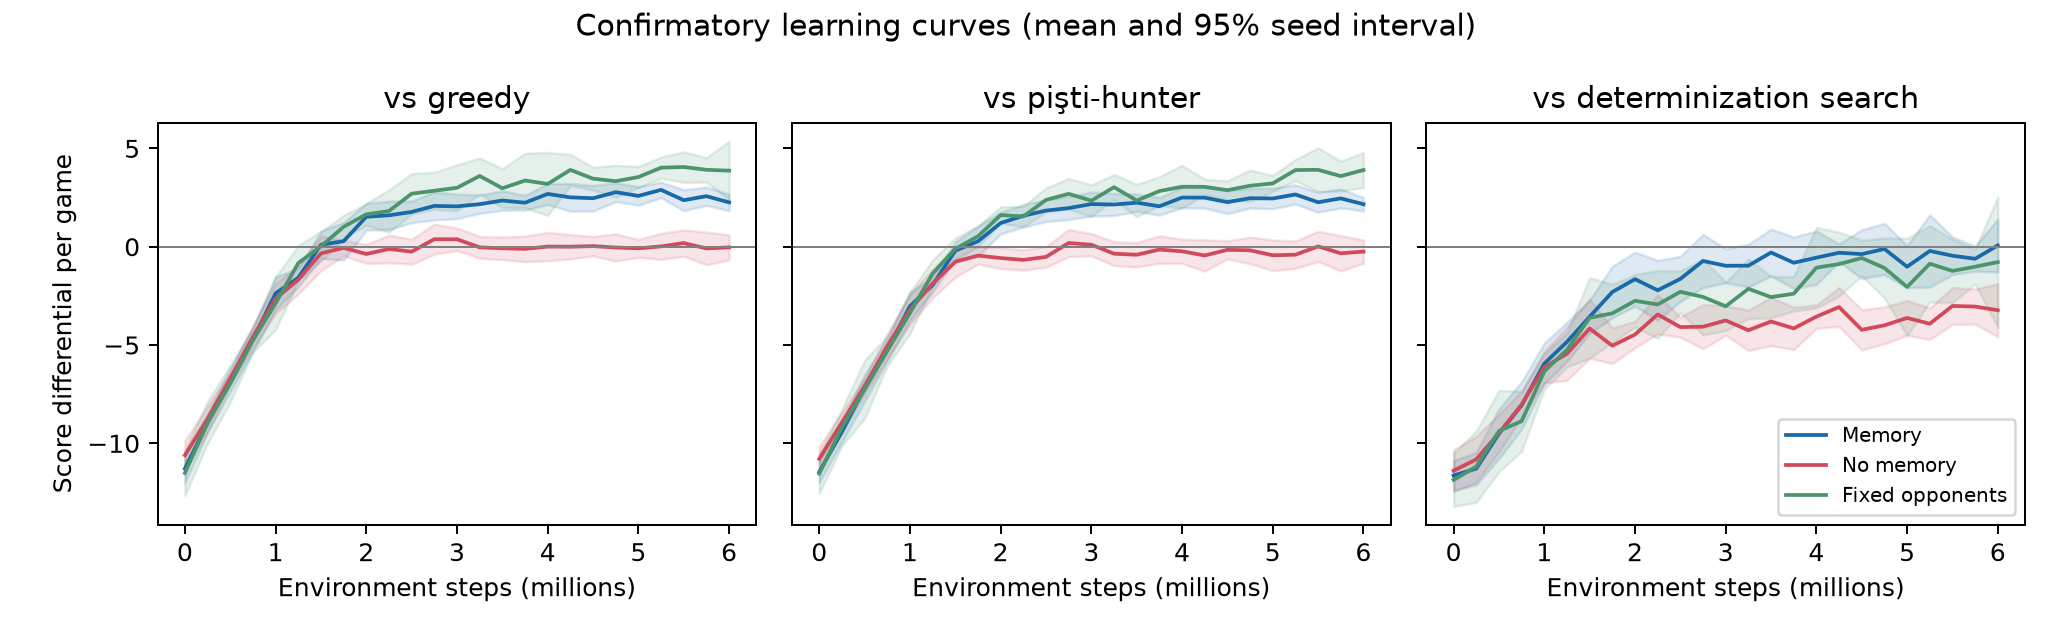
\includegraphics[width=\linewidth]{../plots/study_training_curves.png}
    \caption{Learning curves against three common anchors. Lines are means across ten seeds for each memory condition and five seeds for the fixed-opponent control; bands are 95\% $t$ intervals over training seeds.}
    \label{fig:training}
\end{figure}
\FloatBarrier

\subsection{Primary memory effect}

\begin{table}[t]
\centering
\caption{Score effects by independent training seed (points per game). Positive values favor memory-on or ordinary memory access.}
\label{tab:memory}
\begin{tabular}{rrrr}
\toprule
Seed & Retrained & Acute removal & Stochastic \\
\midrule
0 & +2.71 & +2.44 & +2.18 \\
1 & +2.78 & +2.73 & +2.66 \\
2 & +2.94 & +2.79 & +2.76 \\
3 & +1.96 & +2.99 & +2.10 \\
4 & +2.26 & +1.82 & +2.56 \\
5 & +3.05 & +3.20 & +2.33 \\
6 & +2.87 & +3.07 & +2.29 \\
7 & +2.85 & +2.83 & +2.46 \\
8 & +2.74 & +1.80 & +1.93 \\
9 & +2.42 & +2.67 & +2.56 \\
\midrule
Mean & +2.66 & +2.63 & +2.38 \\
\bottomrule
\end{tabular}
\end{table}


The ten seed-matched deterministic comparisons gave a mean memory-on minus memory-off effect of \DirectMean{} points per game (median \DirectMedian{}; seed-level 95\% $t$ interval [\DirectCILow{}, \DirectCIHigh{}]; crossed seed/deal bootstrap interval [\DirectBootLow{}, \DirectBootHigh{}]). \DirectPositive{} of ten seed effects were positive and the exact two-sided sign-flip test gave $p=\DirectP$. The aggregate memory-on win rate was \DirectWinRate{}, with \DirectPistiDiff{} additional pişti events and \DirectCapturedDiff{} additional captured cards per game relative to memory-off. The estimate is large by the preregistered descriptive threshold, both intervals exclude zero, and the smallest seed effect remains positive. We therefore support H1 for the tested architecture, curriculum, and training budget.

\subsection{Acute removal, adaptation, and sensitivity}

Zeroing \code{seen} only at inference changed the memory-trained policy's score by \AcuteMean{} points per game (95\% interval [\AcuteCILow{}, \AcuteCIHigh{}], $p=\AcuteP$; \AcutePositive{}/10 positive seeds). The acute-minus-retrained contrast was \AdaptMean{} points per game ($p=\AdaptP$). Thus H2 is supported: trained policies consistently rely on the feature. H3 is not supported as a directional claim. Acute removal was only 0.02 points less damaging than retraining without memory, with four of ten within-seed contrasts positive; the data indicate near equality rather than detectable compensation through no-memory training.

With stochastic action sampling, the retrained contrast was \StochasticMean{} points per game (95\% interval [\StochasticCILow{}, \StochasticCIHigh{}], $p=\StochasticP$). Averaged over greedy, hunter, and determinization-search anchors, the on-minus-off effect was \AnchorMean{} points per game ($p=\AnchorP$). The cross-play rating difference averaged \RatingDiff{} Elo-like points in favor of memory-on. The stochastic and common-opponent analyses therefore preserve the sign, seed consistency, and large descriptive magnitude of the direct result; cross-play provides a separate descriptive ranking check rather than another independent test.

\begin{figure}[t]
    \centering
    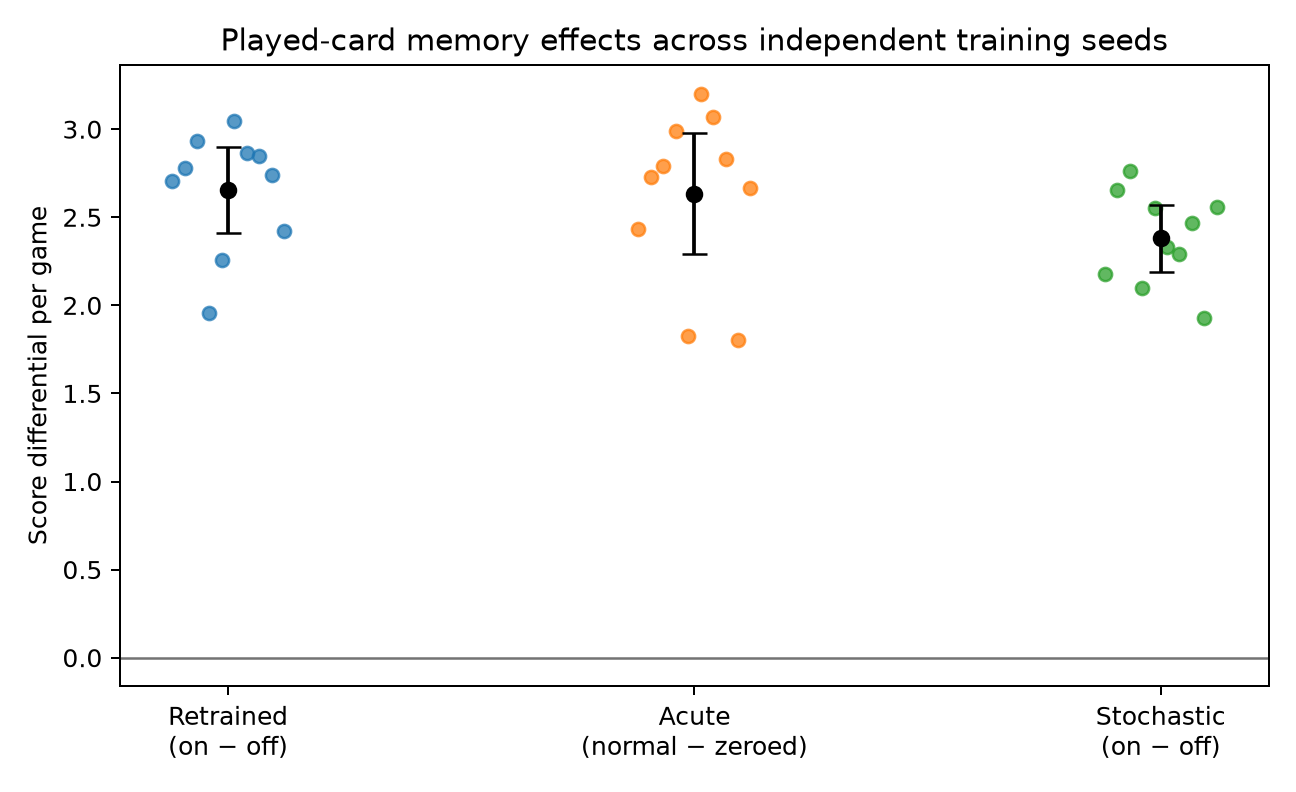
\includegraphics[width=0.82\linewidth]{../plots/memory_study_effects.png}
    \caption{Training-seed effects for retraining, acute feature removal, and stochastic sensitivity. Points are independent training seeds; bars are 95\% $t$ intervals over seeds. Each point averages the same 500 mirrored deal pairs.}
    \label{fig:memory}
\end{figure}

\subsection{League robustness}

\begin{table}[t]
\centering
\caption{Discovered attack edges for paired targets (points per game). Larger values indicate a more successful fixed-budget attack.}
\label{tab:robustness}
\begin{tabular}{rrrrr}
\toprule
Target seed & Attacker seed & League & Fixed & Fixed $-$ league \\
\midrule
0 & 100 & +0.98 & +0.65 & -0.33 \\
1 & 101 & +0.27 & -0.03 & -0.29 \\
2 & 102 & +0.76 & +0.85 & +0.09 \\
3 & 103 & +1.23 & +0.17 & -1.07 \\
4 & 104 & +0.26 & +0.92 & +0.66 \\
\bottomrule
\end{tabular}
\end{table}


Across five paired target seeds, the fixed-minus-league discovered attack edge was \RobustnessMean{} points per game (95\% seed interval [\RobustnessCILow{}, \RobustnessCIHigh{}], exact $p=\RobustnessP$; \RobustnessPositive{}/5 positive pairs). Three attackers against principal league seed 0 found a maximum edge of \PrincipalMax{} points per game. H4 is unsupported: fixed-opponent targets were not consistently easier to attack, and the paired interval spans effects in both directions. The nonzero maximum also demonstrates why these runs cannot certify the principal league policy as unexploitable.

\begin{figure}[t]
    \centering
    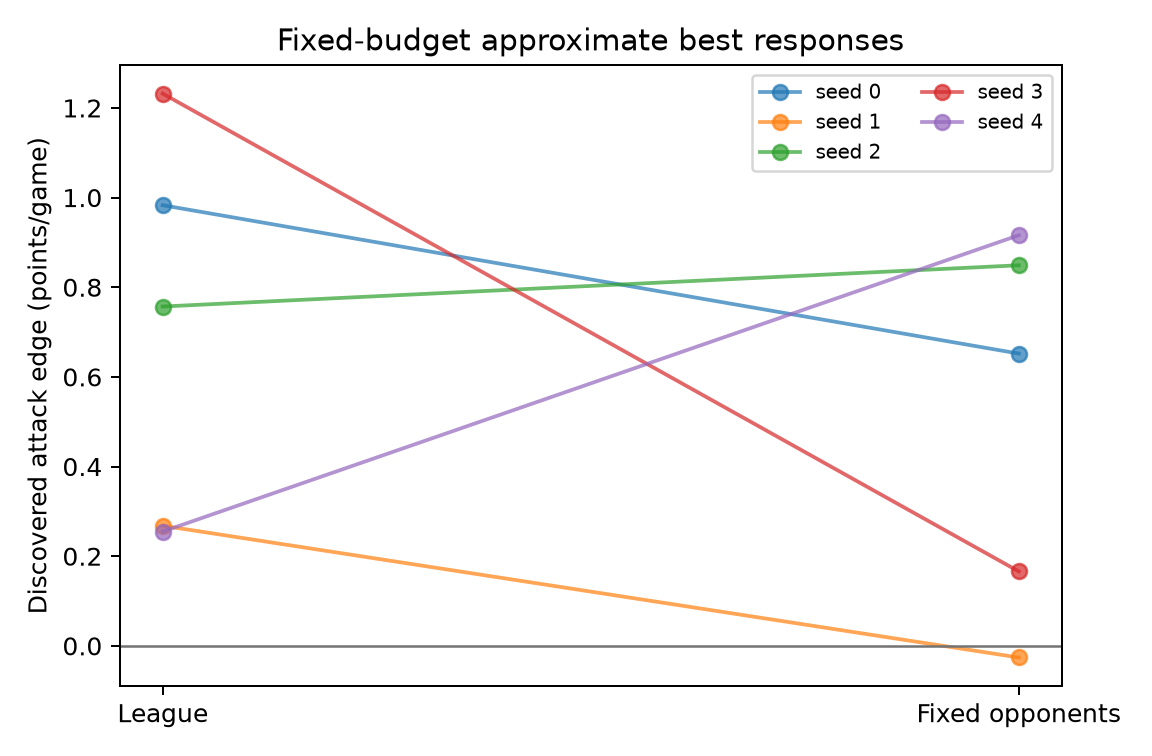
\includegraphics[width=0.72\linewidth]{../plots/robustness_study.png}
    \caption{Fixed-budget attack edges for seed-matched league and fixed-opponent targets. Lines connect targets sharing the same training and attacker seeds. Values are lower bounds on exploitability.}
    \label{fig:robustness}
\end{figure}

\section{Discussion}

The primary result answers the narrow question selected by the discovery process. Exact played-card identity memory was worth approximately 2.7 points per game in direct play, and every independently trained pair favored memory. This is not merely a deterministic-action artifact: stochastic evaluation and three common anchors gave effects of similar magnitude. The effect appears in both pişti creation and card capture, although those secondary decompositions are descriptive and need not sum mechanically to the score difference.

The result does not establish that PPO learned human-style card counting. The engineered vector supplies exact recall of observed identities, and a feed-forward policy may exploit correlations without forming an interpretable count or belief. It establishes a causal representation effect within the paired intervention: when exact identity history is removed while architecture, seed pairing, budget, and evaluation deals are controlled, the resulting policies play substantially worse against their memory-enabled counterparts.

The acute and retrained interventions answer different questions. Acute removal measures how much a learned mapping currently relies on a feature, including distribution shift when a familiar input is zeroed. Retraining measures what the learning system can recover from the remaining observation. A larger acute effect would indicate adaptation: scalar public state and repeated training can substitute for some explicit identity history, even though they do not restore the missing information. A similar pair of effects would instead suggest that the feature supplies information that the selected policy class cannot readily reconstruct or work around.

The benchmark contribution is intentionally modest. PPO, snapshot leagues, determinization search, and learned attacks are established techniques. The value here is a controlled traditional-game case study, deal-paired evaluation, transparent uncertainty over training runs, and code that makes information ownership explicit. The absence of a directly relevant \pisti{} AI paper in our structured search supports domain novelty only under that protocol; it is not proof that no such work exists.

\subsection{Limitations}

First, ten seeds can identify a stable large effect but still give a broad interval for heterogeneous or small effects. The exact permutation test also has discrete resolution. Second, the treatment removes an engineered identity vector from a feed-forward policy; it does not compare recurrent memory, belief-state models, transformers, or human recall. Third, all training uses one PPO architecture and curriculum. A representation can interact with algorithm, capacity, opponent population, and budget.

Fourth, the search anchor uses independent determinizations and shallow rollouts. It is an honest-information baseline, not ISMCTS and not an upper bound on playing strength. Fifth, a trained attacker only establishes that at least one profitable response was or was not found under a fixed optimizer, initialization, and budget. Even replicated nonpositive edges cannot establish equilibrium. Sixth, the opening-Jack procedure and Jack-on-Jack bonus select explicit rule variants; results should not be assumed to transfer unchanged to every household convention, multiplayer partnership play, or 151-point matches. Finally, we did not run human evaluation. Claims about human-recognizable card counting, practical expertise, or cultural authenticity require expert players and an appropriate participant protocol.

\subsection{Implications and next experiments}

The next informative experiment is not simply a larger version of the same run. If the memory effect is stable, a representation ladder should compare exact \code{seen}, rank-count compression, a recurrent policy receiving only events, and a learned belief state. This would distinguish information content from inductive bias and input dimension. If the effect is unstable, increasing seeds and crossing memory with training population is more valuable than adding algorithms. In either case, an OpenSpiel port and exact analysis of reduced \pisti{} subgames would provide calibrated exploitability checks, while ISMCTS would be the appropriate stronger search baseline. Human comparison should be attempted only after the computational hypotheses and rule variants are fixed.

\section{Conclusion}

In this seed-replicated \pisti{} experiment, explicit played-card memory produced a large and consistent advantage: \DirectMean{} points per game across ten paired training seeds, with all ten effects positive. Acute feature removal produced almost the same loss, and stochastic and common-anchor evaluations corroborated the direction. The fixed-budget attack study did not support the separate hypothesis that the snapshot league yielded harder-to-attack policies than fixed-opponent training. These findings support explicit memory as an important input for the tested feed-forward PPO system while leaving human-level play, algorithm independence, and equilibrium convergence unresolved.

More broadly, the study illustrates a practical sequence for turning an exploratory software project into research: audit claims against artifacts, review adjacent literature, choose a discriminating question, freeze the protocol, represent training variation, preserve chance pairing, and weaken conclusions when the measurement cannot support them. That process changed both the implementation and the question before it changed the prose.

\section*{Data, code, and ethics statement}

The repository contains the engine, resolved configurations, exact direct dependency versions, model checksums, deal-level evaluation records, analysis programs, generated tables, and protocol amendments needed to audit the study. The checksum manifest identifies the final artifacts. No human participants or personal data were used. The work evaluates a computational implementation of a traditional game and does not claim to validate human expertise or represent all regional rule conventions.

\bibliographystyle{plain}
\bibliography{references}

\appendix
\section{Reproduction map}

The paired models are produced by \path{scripts/run_memory_study.sh}; fixed controls by \path{scripts/run_fixed_controls.sh}; deterministic, acute, stochastic, anchor, and cross-play records by \path{scripts/run_study_evaluation.sh}; and fixed-budget attacks by \path{scripts/run_robustness_study.sh}. The modules \path{analysis.memory_study}, \path{analysis.robustness_study}, and \path{analysis.paper_assets} generate summaries, figures, and manuscript tables. Each main match retains both game records for every deal.

\section{Hypotheses and decision rules}

H1 predicts a positive retrained memory effect and is primary. H2 predicts a positive acute effect. H3 predicts acute removal is at least as damaging as retraining without memory because the latter can adapt. H4 predicts that fixed-budget attackers find a smaller edge against league targets than against fixed-opponent targets. H2--H4 are secondary. Deal-only significance is never used to promote a seed-unstable effect, and failure to find an attack is not interpreted as zero exploitability.

\end{document}
